\begin{figure}[htbp]
\centering
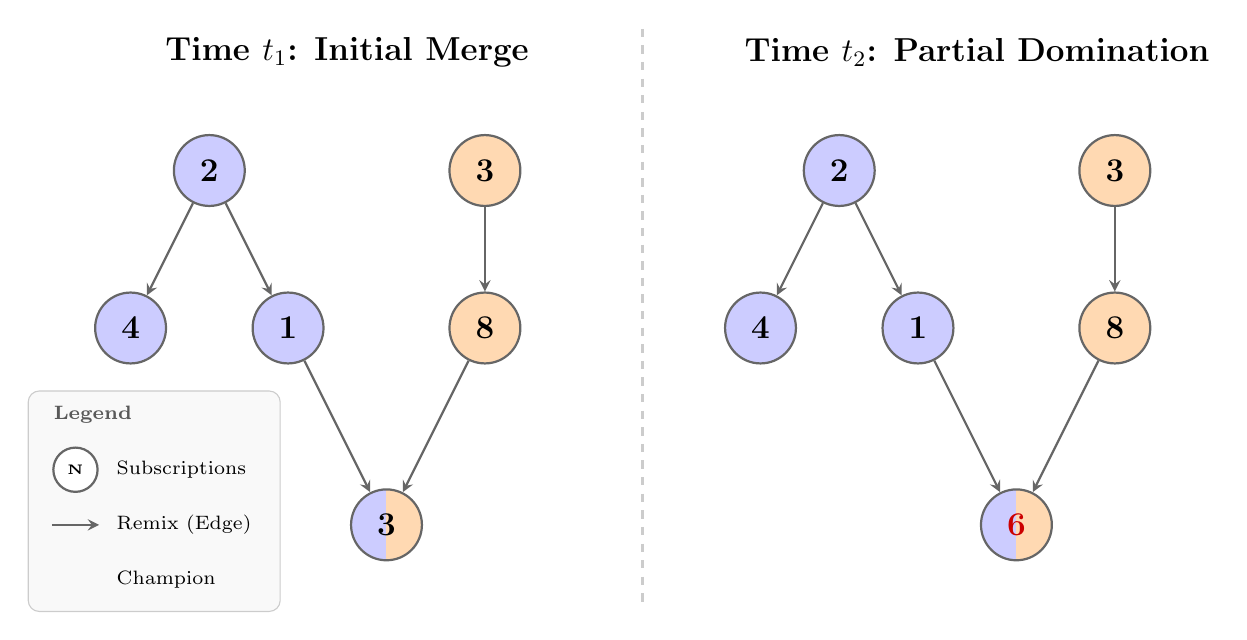
\begin{tikzpicture}[
    >=stealth,
    bluenode/.style={circle, draw=black!60, thick, fill=blue!20, minimum size=0.9cm, font=\large\bfseries},
    orangenode/.style={circle, draw=black!60, thick, fill=orange!30, minimum size=0.9cm, font=\large\bfseries},
    combonode/.style={circle, draw=black!60, thick, minimum size=0.9cm, font=\large\bfseries,
        path picture={
            \fill[blue!20] (path picture bounding box.south west) rectangle (path picture bounding box.north);
            \fill[orange!30] (path picture bounding box.south) rectangle (path picture bounding box.north east);
        }
    },
    edge/.style={->, thick, gray!80!black},
    champlabel/.style={font=\small\bfseries}
]

% ===== Left Side: Initial Merge =====
\node[font=\large\bfseries] at (-3.75, 3.5) {Time $t_1$: Initial Merge};

% Blue graph (forked)
\node[bluenode] (bl_root) at (-5.5, 2) {2};
\node[bluenode] (bl_c1) at (-6.5, 0) {4};
\node[bluenode] (bl_c2) at (-4.5, 0) {1};
\draw[edge] (bl_root) -- (bl_c1);
\draw[edge] (bl_root) -- (bl_c2);

% Orange graph
\node[orangenode] (or_root) at (-2.0, 2) {3};
\node[orangenode] (or_c1) at (-2.0, 0) {8};
\draw[edge] (or_root) -- (or_c1);

% Combination node
\node[combonode] (combo_L) at (-3.25, -2.5) {3};
\draw[edge] (bl_c2) -- (combo_L);
\draw[edge] (or_c1) -- (combo_L);

% Champions Left
\node[text=blue!80!black, font=\Large] at ([xshift=-12pt, yshift=12pt]bl_c1.north west) {$\bigstar$};
\node[text=orange!80!black, font=\Large] at ([xshift=12pt, yshift=12pt]or_c1.north east) {$\bigstar$};


% ===== Right Side: Partial Domination =====
\node[font=\large\bfseries] at (4.25, 3.5) {Time $t_2$: Partial Domination};

% Blue graph (forked)
\node[bluenode] (br_root) at (2.5, 2) {2};
\node[bluenode] (br_c1) at (1.5, 0) {4};
\node[bluenode] (br_c2) at (3.5, 0) {1};
\draw[edge] (br_root) -- (br_c1);
\draw[edge] (br_root) -- (br_c2);

% Orange graph
\node[orangenode] (or_root_R) at (6.0, 2) {3};
\node[orangenode] (or_c1_R) at (6.0, 0) {8};
\draw[edge] (or_root_R) -- (or_c1_R);

% Combination node
\node[combonode] (combo_R) at (4.75, -2.5) {\textcolor{red!80!black}{6}};
\draw[edge] (br_c2) -- (combo_R);
\draw[edge] (or_c1_R) -- (combo_R);

% Champions Right
\node[text=blue!80!black, font=\Large] at ([xshift=-12pt, yshift=12pt]combo_R.north west) {$\bigstar$};
\node[text=orange!80!black, font=\Large] at ([xshift=12pt, yshift=12pt]or_c1_R.north east) {$\bigstar$};

% Separation line
\draw[dashed, thick, gray!40] (0, 3.8) -- (0, -3.5);

% ===== Legend =====
\begin{scope}[shift={(-7.8, -0.8)}]
    \draw[rounded corners=4pt, fill=gray!5, draw=gray!40] (0, 0) rectangle (3.2, -2.8);
    \node[anchor=west, font=\scriptsize\bfseries, text=gray!70!black] at (0.2, -0.3) {Legend};
    
    \node[circle, draw=black!60, thick, fill=white, minimum size=0.4cm, font=\tiny\bfseries] at (0.6, -1.0) {N};
    \node[anchor=west, font=\scriptsize] at (1.0, -1.0) {Subscriptions};
    
    \draw[->, thick, gray!80!black] (0.3, -1.7) -- (0.9, -1.7);
    \node[anchor=west, font=\scriptsize] at (1.0, -1.7) {Remix (Edge)};
    
    \node[text=gray!60!black, font=\large] at (0.6, -2.4) {$\bigstar$};
    \node[anchor=west, font=\scriptsize] at (1.0, -2.4) {Champion};
\end{scope}

\end{tikzpicture}
\caption{Label inheritance and partial domination. Labels are represented by colors (e.g., blue and orange). Subscription counts are shown inside the nodes. \textbf{Left ($t_1$):} A combination node merges a proposal from the blue label (1~sub) and the orange label (8~subs), inheriting both labels. With 3~subscriptions, it is not the champion of either label. \textbf{Right ($t_2$):} The combination node gains subscriptions, reaching 6. This exceeds the highest-ranked pure blue proposal (4~subs), making the combination the new champion of the blue label. However, it still trails the highest-ranked pure orange proposal (8~subs), which remains the orange champion. The combination thus dominates the ballot slot for one of its labels but not the other.}
\label{fig:label-domination}
\end{figure}
